\begin{frame}[fragile]
\frametitle{If you've ever googled any of these\ldots}
\begin{block}{You probably got an answer as sensible as this}
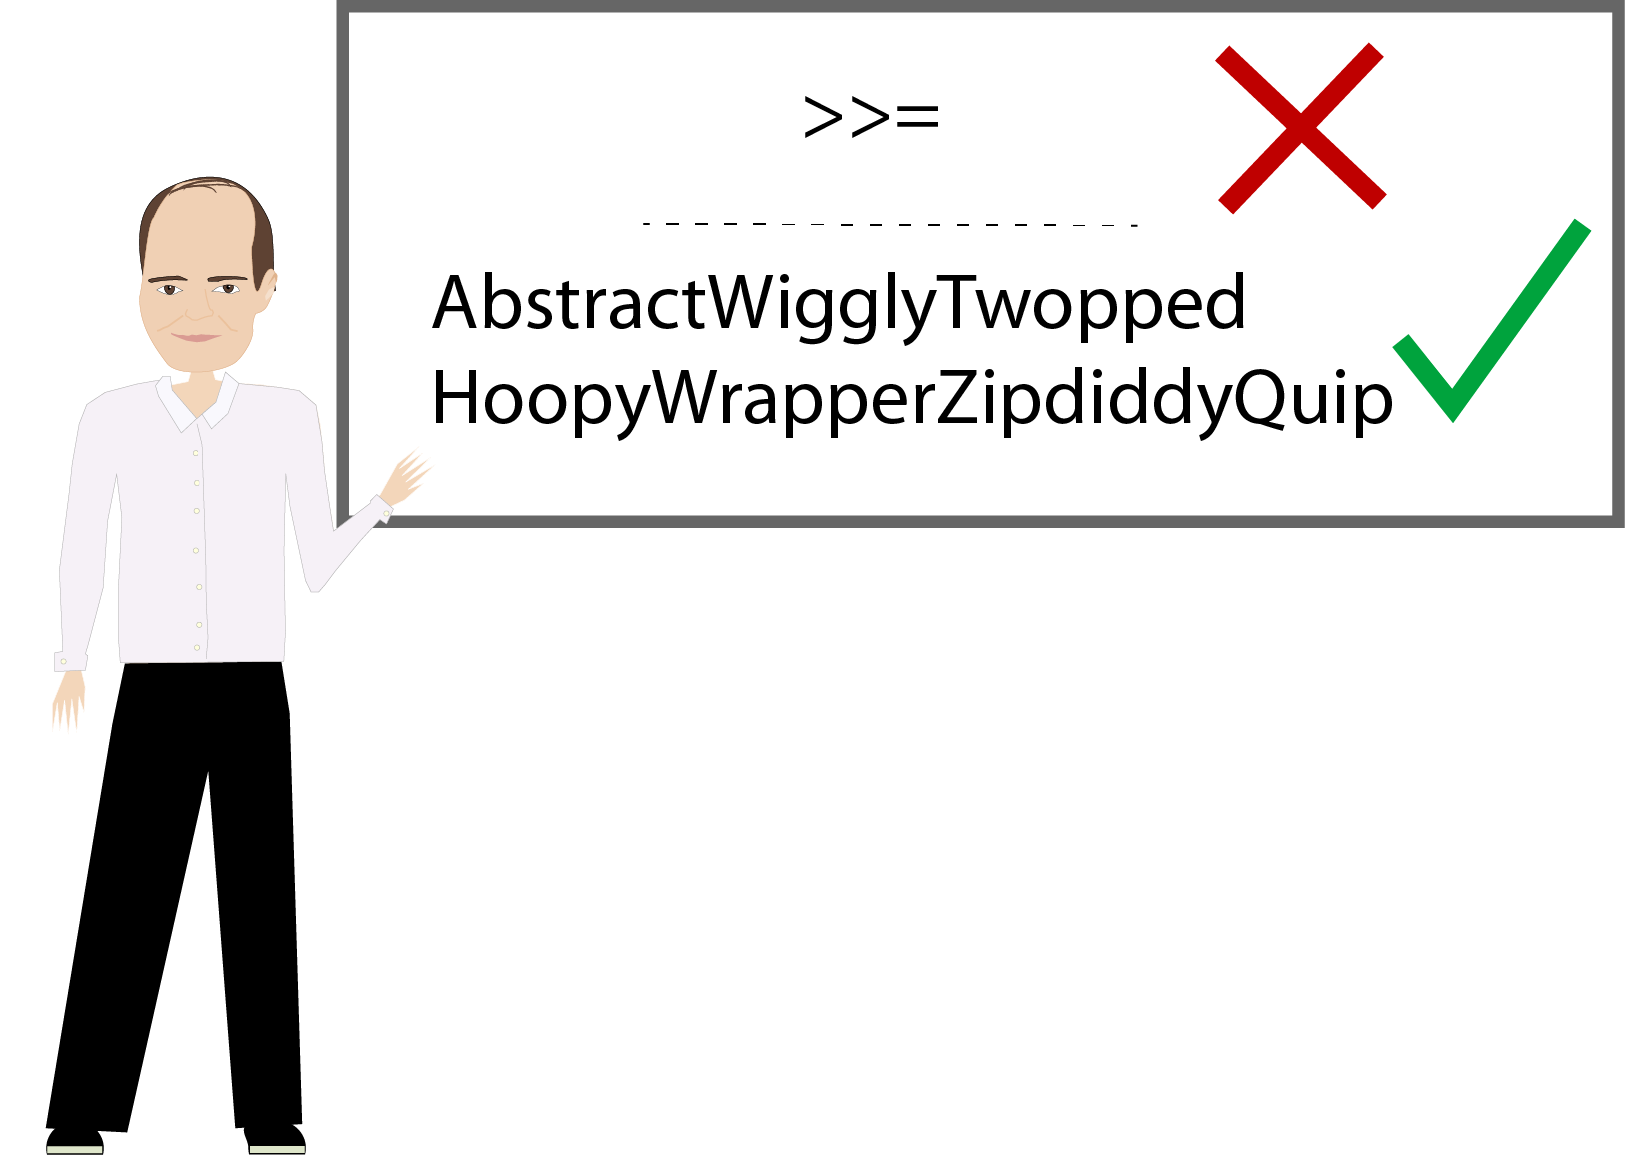
\includegraphics[height=3.8cm]{image/AbstractWigglyTwoppedHoopyWrapperZipdiddyQuip.png}
\end{block}
\end{frame}

\begin{frame}
\frametitle{Goals}
\begin{itemize}
\item<1-> Emphasis on the \emph{practical motivations} for the specific structures.
\item<2-> This is not about the details of concepts like monads.
\item<3-> This is about the process of reasoning that leads to their discovery.
\end{itemize}
\end{frame}

\begin{frame}
\frametitle{Goals}
\begin{block}{Nothing I tell you pertains to any specific programming language.}
\begin{itemize}
\item Java
\item Python
\item JavaScript
\item \emph{doesn't matter, it still applies}
\end{itemize}
\end{block}
\end{frame}

\begin{frame}
\frametitle{Goals}
\begin{block}{There is no emphasis on a specific type of programming.}
\begin{itemize}
\item Functional
\item Dysfunctional
\item Object-disoriented
\item Dynamically-typed
\item Hacking it out like a drunk dog muffin
\item \emph{it's all the same}
\end{itemize}
\end{block}
\end{frame}
